\subsection{Stichprobe}
Es nahmen 23 Studierende der Eberhard Karls Universität Tübingen an der Untersuchung teil. Die Stichprobe bestand aus 11 Männern und 12 Frauen im Alter von 19 bis 28 Jahren (\textit{M}= 21.5). Die Probanden nahme im Rahmen einer Lehrveranstaltung an der Studie teil und erhielten keine Vergütung für ihre Teilnahme. Die Versuchteilnehmer waren naiv gegenüber der Fragestellung und waren alle entweder normalsichtig oder trugen eine entsprechende Sehhilfe. Drei der Probanden waren Linkshänder. Alle Versuchspersonen unterzeichneten eine Einverständniserklärung zur Teilnahme an dem Versuch.

\subsection{Materialien}
Das Experiment wurde an einem DOS Computer durchgeführt. 
Zur Darstellung wurde ein Standard-VGA-Röhrenbildschirm verwendet. Der Abstand der Versuchspersonen zum Bildschirm betrug circa 57 cm. Das Experiment wurde mit der Software ''Experimental Runtime System'' der Firma Berisoft programmiert und durchgeführt. Die Reaktionszeiten wurden mit zwei seperaten Reaktionszeitmessern mit einer geringen Latenz gemessen. Zur Präsentation der auditiven Reize wurde ein Paar handelsüblicher Kopfhörer verwendet.
\begin{figure*}[t]
	\centering
  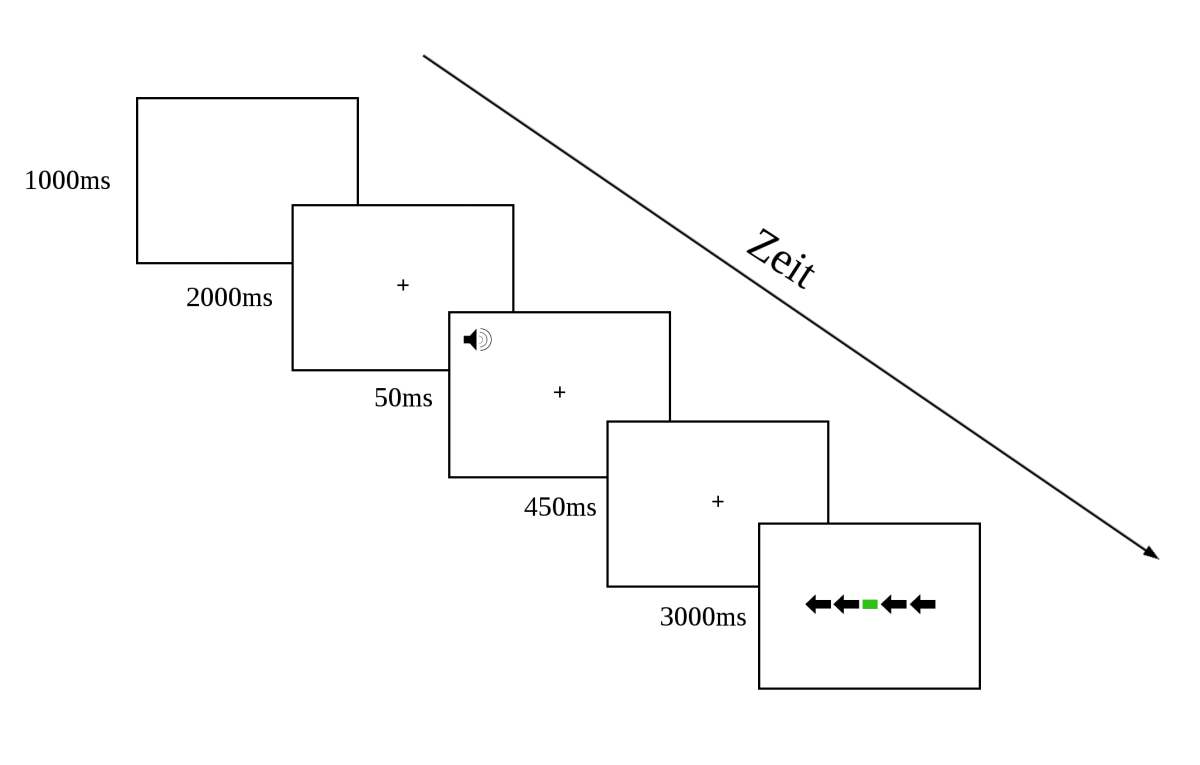
\includegraphics[width=\textwidth]{grafiken/Ablauf.png}
	\caption{Beispiel eines typischen Trials mit auditivem Hinweisreiz.}
	\label{fig:ablauf}
\end{figure*}
\subsection{Versuchsdurchführung}
Zu Beginn jedes Durchgangs wurde den Versuchspersonen 2000 Milisekunden ein weißes Fixationskreuz (Luminanz: $40.1 cd/m^2$) der Größe 0.6°x0.6° auf der Mitte des schwarzen Bildschirms (Luminanz: $< 0.1cd/m^2$) präsentiert. In der Hälfte der Trials wurden den Versuchspersonen für 50ms ein auditiver Hinweisreiz in Form eines Sinustons ($2000 Hz$, ca. $70dB$) binaural über Kopfhöhrer und anschließend für 450ms wieder ein Fixationskreuz präsentiert. In der anderen Hälfte der Versuchsdurchgängen wurde den Probanden für 500ms ein Fixationskreuz und kein auditiver Hinweisreiz präsentiert.
Anschließend wurde den Versuchspersonen für 3000ms der Zielreiz in der Mitte des Bildschirms dargeboten, der entweder aus einem dunkelgrünen (Luminanz: $8.2 cd/m^2$) oder einem dunkelroten (Luminanz: $9.4 cd/m^2$) Rechteck der Größe 0.4°x0.6° bestand. Umgeben wurde der Zielreiz von vier in regelmäßigen Abständen angeordneten Pfeilen, welche entweder alle nach links oder nach rechts zeigen konnten. Die Größe der Pfeile betrug 0.4°x0.8°.\\
\begin{figure}[t]
	\centering
	 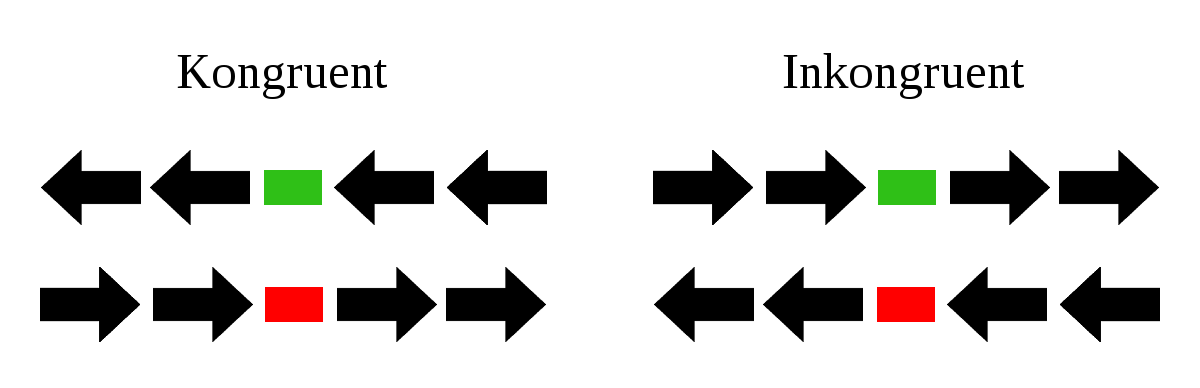
\includegraphics[width=\textwidth]{grafiken/Kongruenz.png}
		\caption{Kongruente und inkongruente Bedingung für Rechte Taste=Rot und Linke Taste=Grün}
		\label{fig:kong} 
\end{figure}
Den Versuchspersonen wurde befohlen den auditiven Reiz, sofern vorhanden, und die Flankierreize zu ignorieren und möglichst schnell auf den Zielreiz zu reagieren. Reagiert werden sollte, indem die Versuchsperson auf die der Farbe zugeordneten Taste drückt. Die Tasten wurden entweder linke Taste für Rot und rechte Taste für Grün oder umgekehrt für alle Blöcke zugeordnet und mussten mit dem Zeigerfinger der entsprechenden Hand bedient werden.\\
Die kongruente Bedingung bestand darin, dass die Richtung der Pfeile mit der Reaktion auf die Pfeile identisch war (z.B. sollte mit der rechten Hand reagiert werden und die Pfeile zeigten nach rechts).
Die inkongruente Bedingung bestand darin, dass die Richtung der Pfeile mit der Reaktion auf die Pfeile nicht identisch war (z.B. sollte mit der rechten Hand reagiert werden und die Pfeile zeigten nach links).\\
Zu Beginn der Studie erhielten die Versuchspersonen eine schriftliche Instruktion und mussten ihre demografischen Daten (Name, Alter, Sehhilfe) angeben. Nach dem sie die Instruktionen gelesen hatten, hatten sie die Möglichkeit, Fragen zu stellen. Anschließend folgte ein Übungsblock mit 24 Durchgängen, nachdem sie nochmals die Möglichkeit hatten Fragen zu stellen. Während des Übungsblocks erhielten die Versuchspersonen ein kurzes Feedback, ob ihre Eingabe korrekt war.\\
Die darauffolgenden 9 Experimentalblöcke bestanden jeweils aus 48 Versuchsdurchgängen. In jedem Block wurde jede der 12 Bedingungen 4 mal in zufälliger Reihenfolge präsentiert. Nach jedem Experimentalblock erhielten die Versuchspersonen ein Feedback über die Anzahl der korrekten Eingaben während des Blocks.\\
Am Ende des Experiments wurden die Probanden über die Hintergründe des Experiments aufgeklärt.

\subsection{Versuchsdesign}
Der Untersuchung liegt ein 2x2x3-faktorielles Design mit Messwiederholung zugrunde. Wir manipulierten dabei die Faktoren Ton (mit oder ohne Ton), Kongruenz zwischen den Zielreizen (kongruent oder inkongruent) und die Distanz der Flankierreize (0.05°, 0.1°, 0.2°).\\
Zusätzlich wurde die Tastenzuordnung, also Reaktionsrichtung auf die Farben, in beiden Möglichkeiten (rechts rot, links grün und rechts grün, links rot) zufällig den Versuchspersonen zugeordnet.\\
Als abhängige Variable wurde die Reaktionszeit und die Fehlerrate erfasst.
